\documentclass[10 pt]{beamer}
\usetheme{Madrid}
\usepackage[utf8]{inputenc}
\usepackage{default}
\usepackage{xspace}
\usepackage{graphicx,graphics} 
\usepackage{color}
\usepackage{amsmath}
\usepackage{amsfonts}
\usepackage{amssymb}
\usepackage{amsthm}
\usepackage{algorithm}
\usepackage{algorithmic}
\usepackage{longtable}
\usepackage{complexity}
\usepackage{tkz-graph}
\usepackage{float}
\usepackage{setspace}

\tikzset{
  LabelStyle/.style = { rectangle, rounded corners, draw,
                       font = \bfseries },
  EdgeStyle/.append style = {-} }
\title{Contention management for Deterministic Networking}

\author{Maël~Guiraud }


\institute[Nokia Bell Labs, DAVID-UVSQ] 
{
  Nokia Bell Labs France - 
  DAVID, Universit\'e de Versailles Saint Quentin\\
}

\subject{Theoretical Computer Science}

\begin{document}

\begin{frame}

  \titlepage
  \centering
  
\includegraphics [width=20mm]{logon.png} \hspace{1cm} 
\includegraphics [width=15mm]{logod.png} \hspace{1cm} 
\includegraphics [width=20mm]{logo.png} \\
\end{frame}

\begin{frame}

  \tableofcontents[]
\end{frame}

\AtBeginSection[]{\begin{frame}

  \small \tableofcontents[currentsection]
\end{frame}
}

\begin{section}{Presentation}

\begin{frame}{Context}
  \centering
  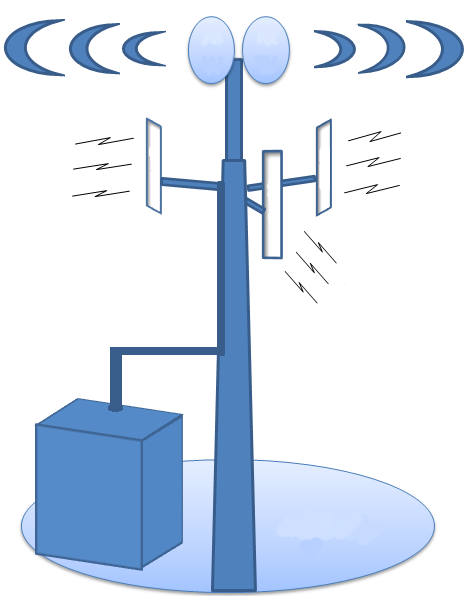
\includegraphics[scale=0.2]{bts.png}\\
  A base transceiver station.

\end{frame}

\begin{subsection}{Introduction}
\begin{frame}{Context}
  \centering
  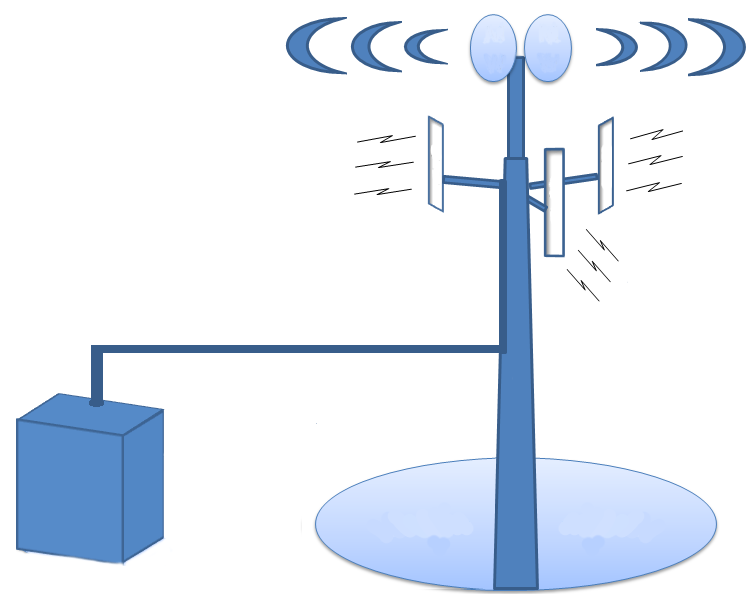
\includegraphics[scale=0.2]{cloudbts.png}\\
  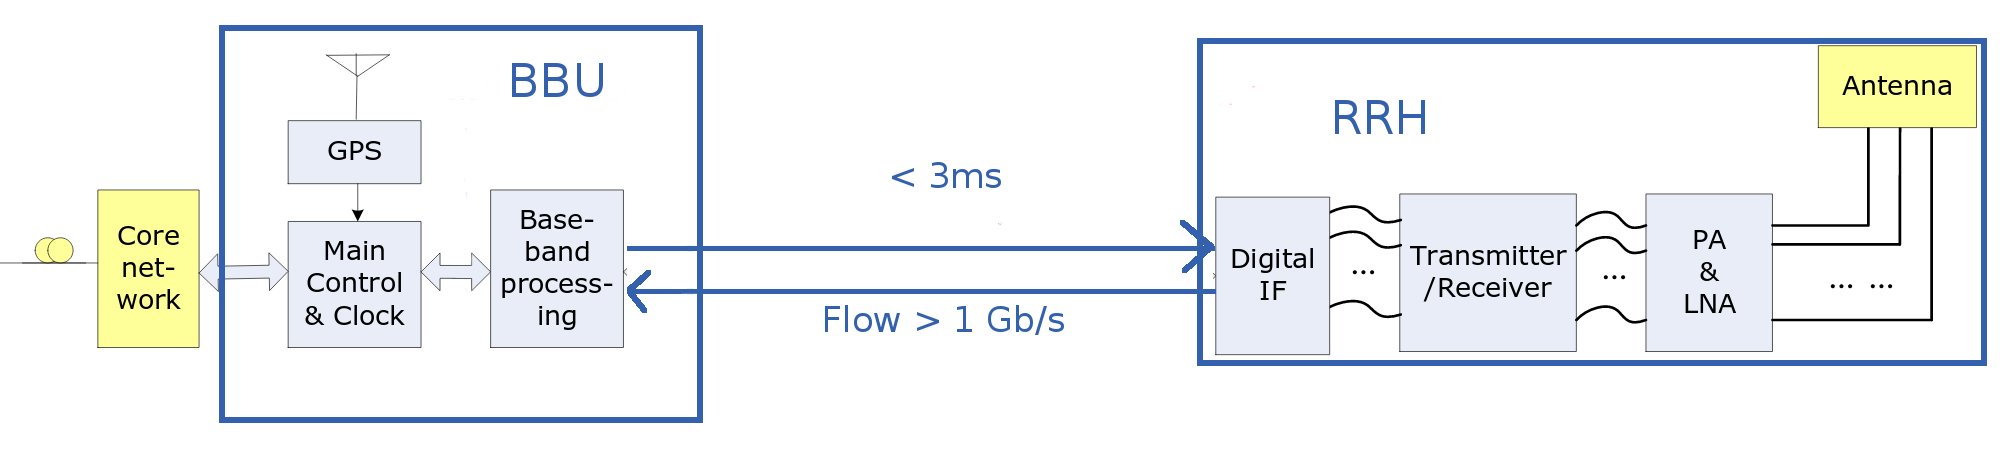
\includegraphics[scale=0.175]{BBURRH.png}
\end{frame}

\begin{frame}{Context}
  \centering
  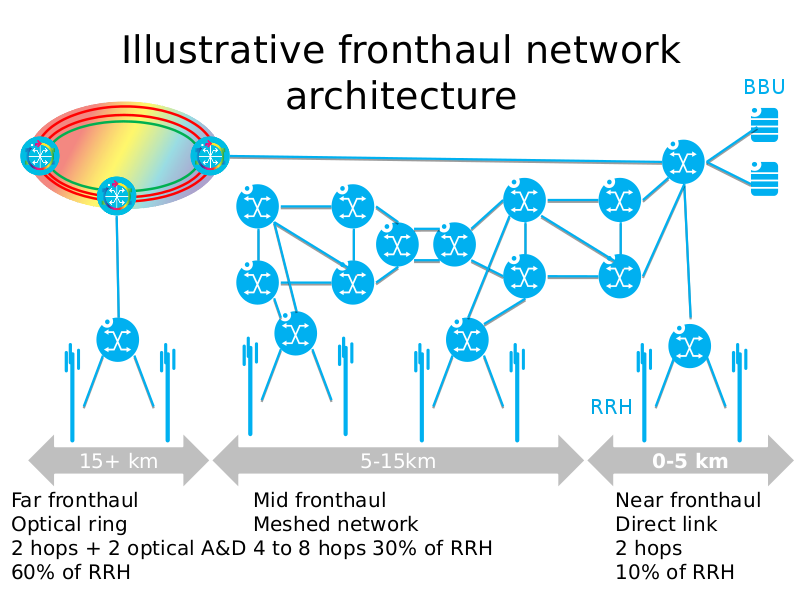
\includegraphics[scale=0.38]{fronthaul0.png}
\end{frame}

% \begin{frame}{Context}
%   \centering
%   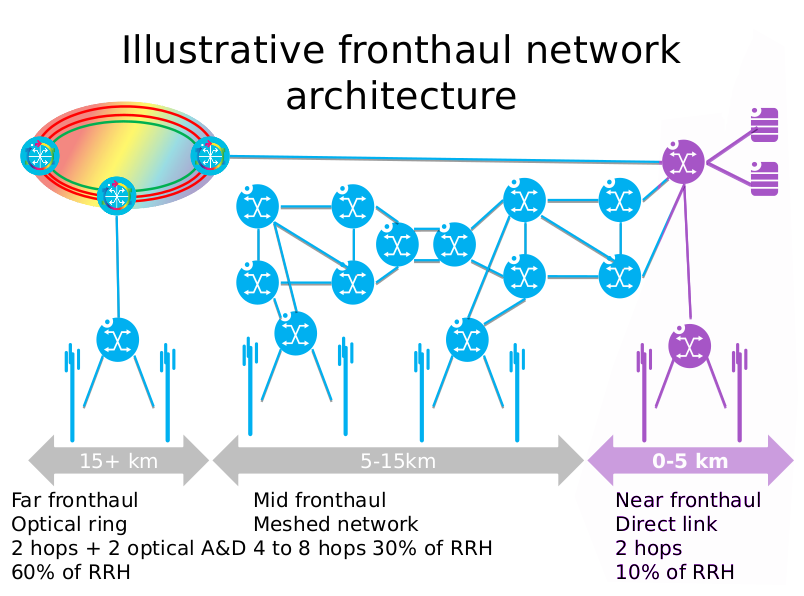
\includegraphics[scale=0.38]{fronthaul.png}
% \end{frame}
\end{subsection}
\begin{subsection}{Model}
\begin{frame}{Model}
\begin{center}
 


\scalebox{0.5}{
\begin{tikzpicture}
  \SetGraphUnit{5}
   \tikzstyle{VertexStyle}=[shape = circle, draw, minimum size = 50pt]
  \Vertex[x=0,y=0]{RRH 3}
  \Vertex[x=0,y=4]{RRH 2}
  \Vertex[x=0,y=8]{RRH 1}
  
  \Vertex[x=16,y=0]{BBU 3}
  \Vertex[x=16,y=4]{BBU 2}
  \Vertex[x=16,y=8]{BBU 1}
  
  \Vertex[x=4,y=4]{Switch 1}
  \Vertex[x=12,y=4]{Switch 2}  
  \tikzset{
  EdgeStyle/.append style = {<-, green} }
  \Edge(BBU 1)(Switch 2)
  \Edge(Switch 1)(RRH 1)
  
  \tikzset{
  EdgeStyle/.append style = {blue} }
  \Edge(BBU 2)(Switch 2)
  \Edge(Switch 1)(RRH 2)
  
  \tikzset{
  EdgeStyle/.append style = {red} }
  \Edge(BBU 3)(Switch 2)
  \Edge(Switch 1)(RRH 3)
  
  \tikzset{
  EdgeStyle/.append style = {black} }
  \Edge(Switch 2)(Switch 1)

\end{tikzpicture}
}

 Network $\rightarrow$ Graph G=(V,A).\\
 \end{center}
\end{frame}


\begin{frame}{Model}
\begin{center}
\scalebox{0.5}{
\begin{tikzpicture}
  \SetGraphUnit{5}
  \tikzstyle{VertexStyle}=[shape = circle, draw, minimum size = 50pt]
  \Vertex[x=0,y=0]{l3}
  \Vertex[x=0,y=4]{l2}
  \Vertex[x=0,y=8]{l1}
  
  \Vertex[x=16,y=0]{s3}
  \Vertex[x=16,y=4]{s2}
  \Vertex[x=16,y=8]{s1}
  
  \Vertex[x=4,y=4]{SL}
  \Vertex[x=12,y=4]{SS}  
  \tikzset{
  EdgeStyle/.append style = {<-,green} }
  \Edge[label = $a_1$](s1)(SS)
  \Edge[label = $b_1$](SL)(l1)
  
  \tikzset{
  EdgeStyle/.append style = {blue} }
  \Edge[label = $a_2$](s2)(SS)
  \Edge[label = $b_2$](SL)(l2)
  
  \tikzset{
  EdgeStyle/.append style = {red} }
  \Edge[label = $a_3$](s3)(SS)
  \Edge[label = $b_3$](SL)(l3)
  
  \tikzset{
  EdgeStyle/.append style = {black} }
  \Edge(SS)(SL)

\end{tikzpicture}
}
\end{center}
\begin{block}{}
 BBU / RRH $\rightarrow$ set of vertices S (sources) and L (leaves).\\

 Physical Delay of a link $\rightarrow$ Weight on arcs.\\
  Slotted time.\\
\end{block}

\end{frame}

% 
% \begin{frame}{Slots}
% 
%    Each links does have a delay in slots corresponding to it's transit time.\\
% 
%   The Flow values in slots correspond to the transmission time.\\
% \vspace{1cm}
%   \centering
%    \begin{tabular}{|c|c|}
%    \hline
%    Period & 19500 slots(1ms) \\
%    \hline
%    1 Flow & 2500 slots\\
%    \hline
%    Range & 0 - 2000 slots\\
%    \hline
%    1 arc & 0 - 700 slots\\
%    \hline
%   \end{tabular}
% 
%   
%   
% \end{frame}
\end{subsection}
\begin{subsection}{Problem}


\begin{frame}{Problem}
  \centering
  
\scalebox{0.5}{
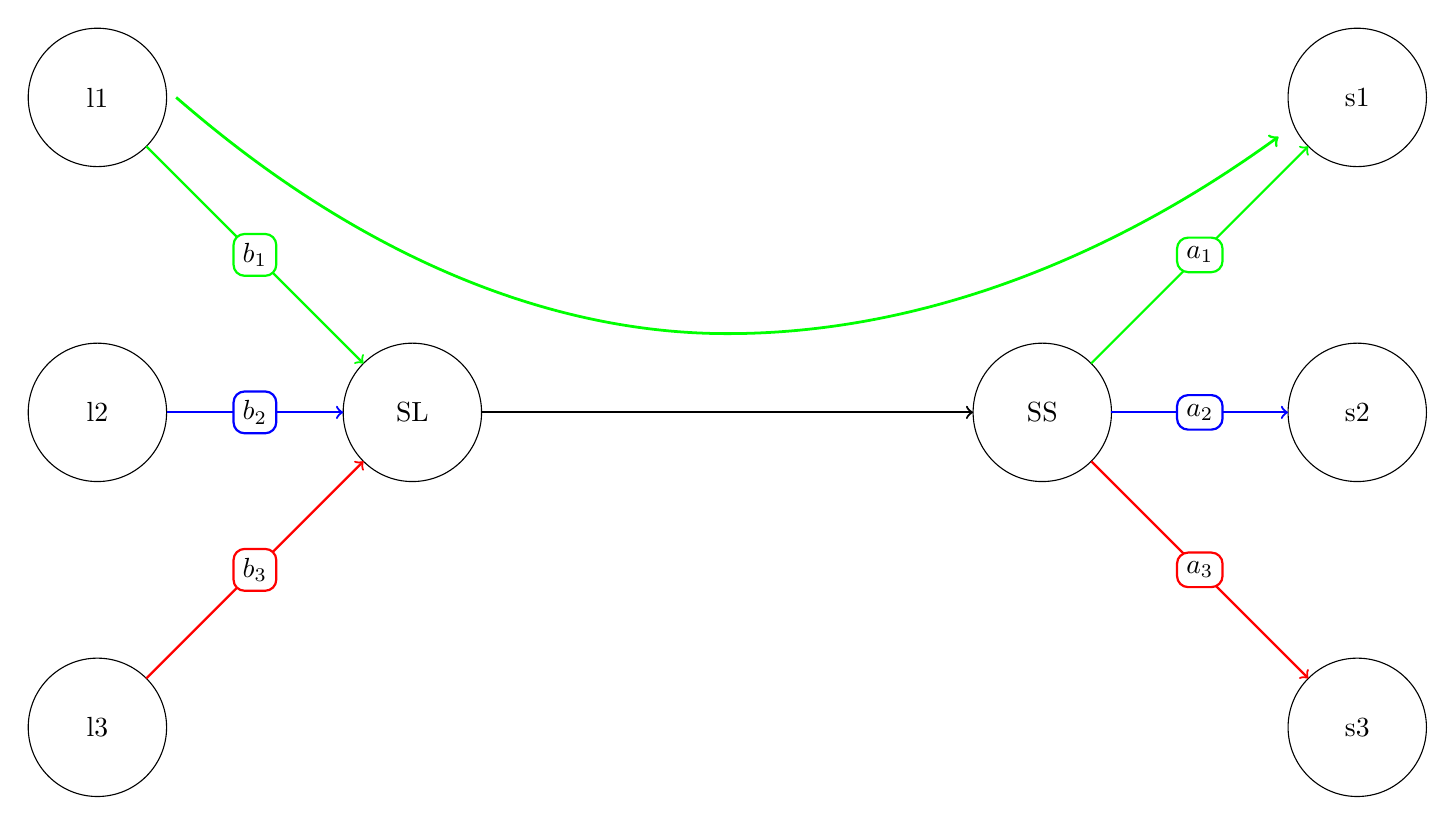
\begin{tikzpicture}
    \SetGraphUnit{5}
  \tikzstyle{VertexStyle}=[shape = circle, draw, minimum size = 50pt]
  \Vertex[x=0,y=0]{l3}
  \Vertex[x=0,y=4]{l2}
  \Vertex[x=0,y=8]{l1}
  
  \Vertex[x=16,y=0]{s3}
  \Vertex[x=16,y=4]{s2}
  \Vertex[x=16,y=8]{s1}
  
  \Vertex[x=4,y=4]{SL}
  \Vertex[x=12,y=4]{SS}  
  \tikzset{
  EdgeStyle/.append style = {<-,green} }
  \Edge[label = $a_1$](s1)(SS)
  \Edge[label = $b_1$](SL)(l1)
  
  \tikzset{
  EdgeStyle/.append style = {blue} }
  \Edge[label = $a_2$](s2)(SS)
  \Edge[label = $b_2$](SL)(l2)
  
  \tikzset{
  EdgeStyle/.append style = {red} }
  \Edge[label = $a_3$](s3)(SS)
  \Edge[label = $b_3$](SL)(l3)
  
  \tikzset{
  EdgeStyle/.append style = {black} }
  \Edge(SS)(SL)

  \draw[->,line width=1pt,green] (1,8) parabola bend (8,5) (15,7.5);


\end{tikzpicture}
}

RRH $\rightarrow$ BBU
\end{frame}



\begin{frame}{Problem}
  \centering
  
\scalebox{0.5}{
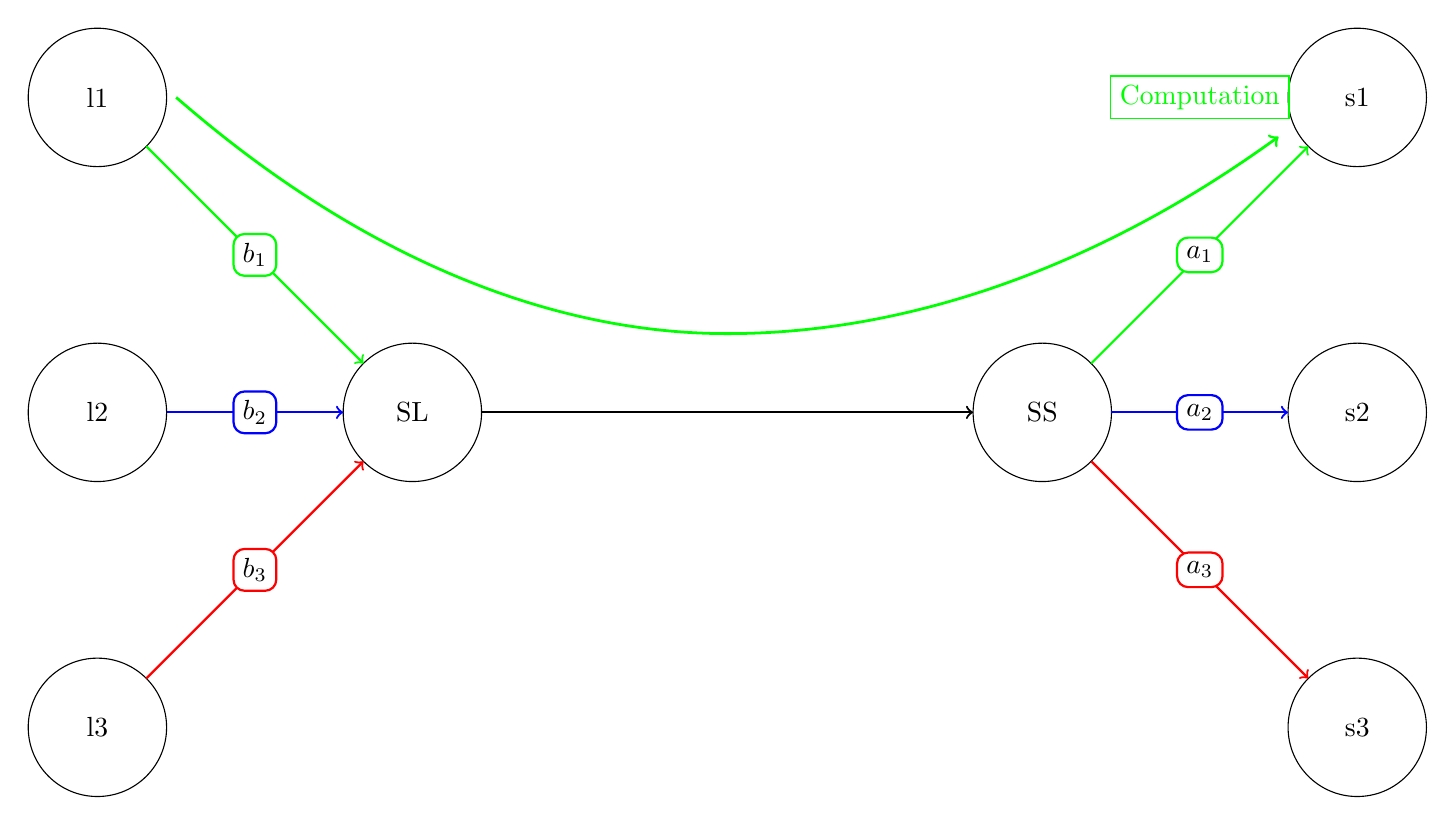
\begin{tikzpicture}
    \SetGraphUnit{5}
  \tikzstyle{VertexStyle}=[shape = circle, draw, minimum size = 50pt]
  \Vertex[x=0,y=0]{l3}
  \Vertex[x=0,y=4]{l2}
  \Vertex[x=0,y=8]{l1}
  
  \Vertex[x=16,y=0]{s3}
  \Vertex[x=16,y=4]{s2}
  \Vertex[x=16,y=8]{s1}
  
  \Vertex[x=4,y=4]{SL}
  \Vertex[x=12,y=4]{SS}  
  \tikzset{
  EdgeStyle/.append style = {<-,green} }
  \Edge[label = $a_1$](s1)(SS)
  \Edge[label = $b_1$](SL)(l1)
  
  \tikzset{
  EdgeStyle/.append style = {blue} }
  \Edge[label = $a_2$](s2)(SS)
  \Edge[label = $b_2$](SL)(l2)
  
  \tikzset{
  EdgeStyle/.append style = {red} }
  \Edge[label = $a_3$](s3)(SS)
  \Edge[label = $b_3$](SL)(l3)
  
  \tikzset{
  EdgeStyle/.append style = {black} }
  \Edge(SS)(SL)

  \draw[->,line width=1pt,green] (1,8) parabola bend (8,5) (15,7.5);
  \node[draw,green] at (14,8) {Computation};



\end{tikzpicture}
}

Computation time
\end{frame}



\begin{frame}{Problem}
  \centering
  
\scalebox{0.5}{
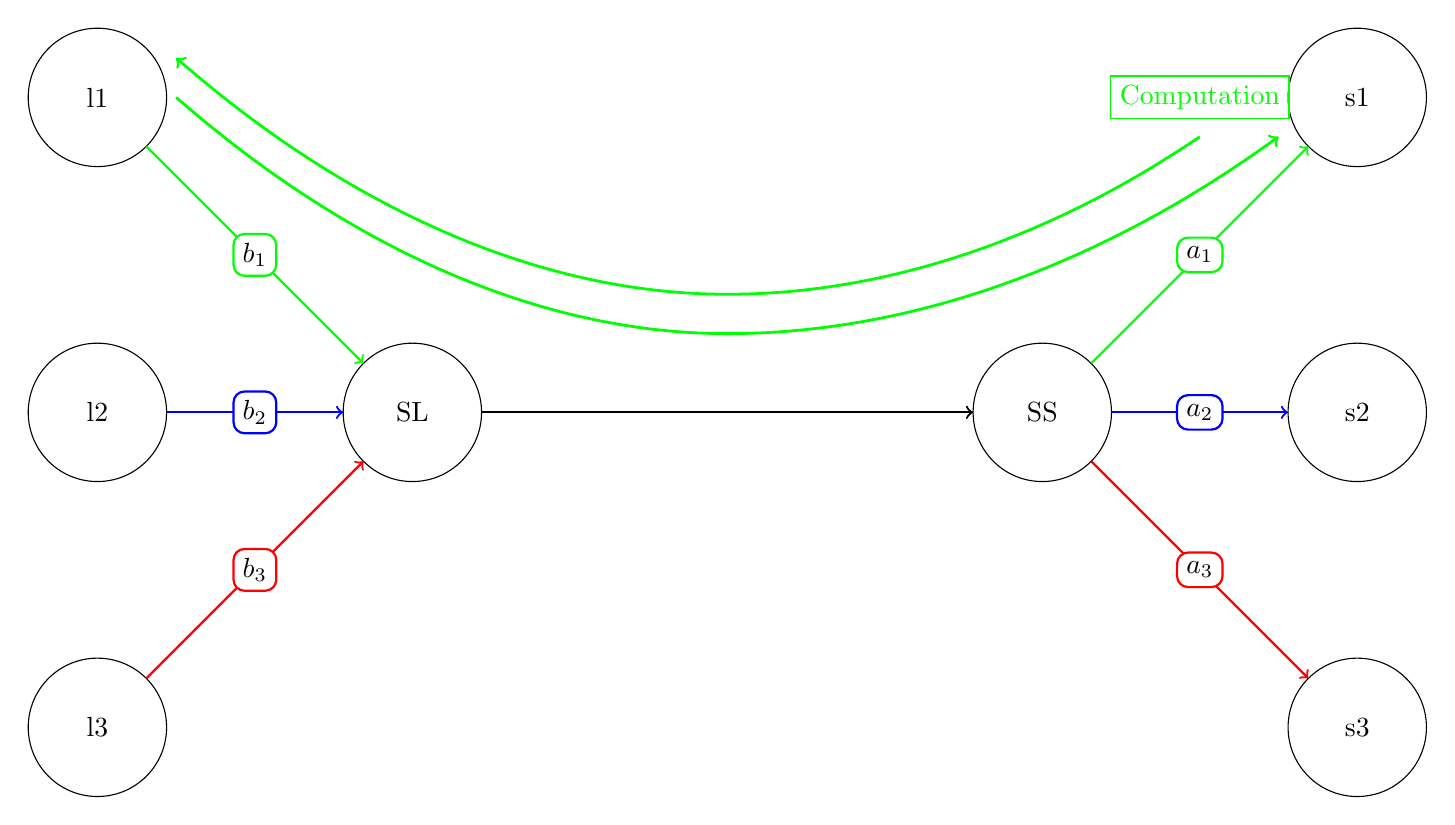
\begin{tikzpicture}
    \SetGraphUnit{5}
  \tikzstyle{VertexStyle}=[shape = circle, draw, minimum size = 50pt]
  \Vertex[x=0,y=0]{l3}
  \Vertex[x=0,y=4]{l2}
  \Vertex[x=0,y=8]{l1}
  
  \Vertex[x=16,y=0]{s3}
  \Vertex[x=16,y=4]{s2}
  \Vertex[x=16,y=8]{s1}
  
  \Vertex[x=4,y=4]{SL}
  \Vertex[x=12,y=4]{SS}  
  \tikzset{
  EdgeStyle/.append style = {<-,green} }
  \Edge[label = $a_1$](s1)(SS)
  \Edge[label = $b_1$](SL)(l1)
  
  \tikzset{
  EdgeStyle/.append style = {blue} }
  \Edge[label = $a_2$](s2)(SS)
  \Edge[label = $b_2$](SL)(l2)
  
  \tikzset{
  EdgeStyle/.append style = {red} }
  \Edge[label = $a_3$](s3)(SS)
  \Edge[label = $b_3$](SL)(l3)
  
  \tikzset{
  EdgeStyle/.append style = {black} }
  \Edge(SS)(SL)
  
  \draw[->,line width=1pt,green] (1,8) parabola bend (8,5) (15,7.5);
  \node[draw,green] at (14,8) {Computation};
  \draw[<-,line width=1pt,green] (1,8.5) parabola bend (8,5.5) (14,7.5);


\end{tikzpicture}
}

BBU $\rightarrow$ RRH\\
\pause
3ms
\end{frame}

\begin{frame}{Problem}
  \centering
  
\scalebox{0.5}{
\begin{tikzpicture}
    \SetGraphUnit{5}
  \tikzstyle{VertexStyle}=[shape = circle, draw, minimum size = 50pt]
  \Vertex[x=0,y=0]{l3}
  \Vertex[x=0,y=4]{l2}
  \Vertex[x=0,y=8]{l1}
  
  \Vertex[x=16,y=0]{s3}
  \Vertex[x=16,y=4]{s2}
  \Vertex[x=16,y=8]{s1}
  
  \Vertex[x=4,y=4]{SL}
  \Vertex[x=12,y=4]{SS}  
  \tikzset{
  EdgeStyle/.append style = {<-,green} }
  \Edge[label = $a_1$](s1)(SS)
  \Edge[label = $b_1$](SL)(l1)
  
  \tikzset{
  EdgeStyle/.append style = {blue} }
  \Edge[label = $a_2$](s2)(SS)
  \Edge[label = $b_2$](SL)(l2)
  
  \tikzset{
  EdgeStyle/.append style = {red} }
  \Edge[label = $a_3$](s3)(SS)
  \Edge[label = $b_3$](SL)(l3)
  
  \tikzset{
  EdgeStyle/.append style = {black} }
  \Edge(SS)(SL)

\end{tikzpicture}
}

  Scheduling the messages
  \begin{itemize}
   \item No collisions on switches
   \item Periodicity
  \end{itemize}

 
\end{frame}
\end{subsection}
\begin{subsection}{Goal}
\begin{frame}{Tools}
  \centering
  
\scalebox{0.5}{
\begin{tikzpicture}
  
  \SetGraphUnit{5}
  \tikzstyle{VertexStyle}=[shape = circle, draw, minimum size = 50pt]
  \Vertex[x=0,y=0]{l3}
  \Vertex[x=0,y=4]{l2}
  \Vertex[x=0,y=8]{l1}
  
  \Vertex[x=16,y=0]{s3}
  \Vertex[x=16,y=4]{s2}
  \Vertex[x=16,y=8]{s1}
  
  \Vertex[x=4,y=4]{SL}
  \Vertex[x=12,y=4]{SS}  
  \tikzset{
  EdgeStyle/.append style = {<-,green} }
  \Edge[label = $a_1$](s1)(SS)
  \Edge[label = $b_1$](SL)(l1)
  
  \tikzset{
  EdgeStyle/.append style = {blue} }
  \Edge[label = $a_2$](s2)(SS)
  \Edge[label = $b_2$](SL)(l2)
  
  \tikzset{
  EdgeStyle/.append style = {red} }
  \Edge[label = $a_3$](s3)(SS)
  \Edge[label = $b_3$](SL)(l3)
  
  \tikzset{
  EdgeStyle/.append style = {black} }
  \Edge(SS)(SL)
  \node (0) at (1,-1){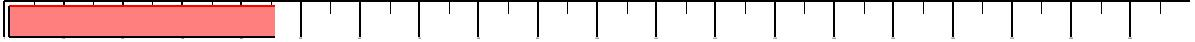
\includegraphics[scale=0.1]{chronogrames/0.jpeg}};
  \node (1) at (1,3){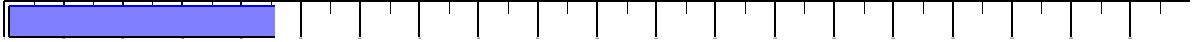
\includegraphics[scale=0.1]{chronogrames/1.jpeg}};
  \node (2) at (1,7){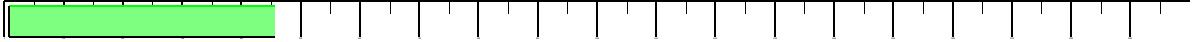
\includegraphics[scale=0.1]{chronogrames/2.jpeg}};
  \node (2) at (4,5){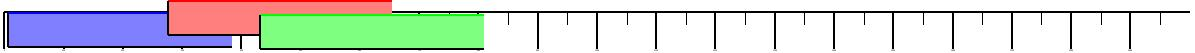
\includegraphics[scale=0.15]{chronogrames/3.jpeg}};
\end{tikzpicture}
}

\end{frame}


\begin{frame}{Tools}
  \centering
  
\scalebox{0.5}{
\begin{tikzpicture}
    \SetGraphUnit{5}
  \tikzstyle{VertexStyle}=[shape = circle, draw, minimum size = 50pt]
  \Vertex[x=0,y=0]{l3}
  \Vertex[x=0,y=4]{l2}
  \Vertex[x=0,y=8]{l1}
  
  \Vertex[x=16,y=0]{s3}
  \Vertex[x=16,y=4]{s2}
  \Vertex[x=16,y=8]{s1}
  
  \Vertex[x=4,y=4]{SL}
  \Vertex[x=12,y=4]{SS}  
  \tikzset{
  EdgeStyle/.append style = {<-,green} }
  \Edge[label = $a_1$](s1)(SS)
  \Edge[label = $b_1$](SL)(l1)
  
  \tikzset{
  EdgeStyle/.append style = {blue} }
  \Edge[label = $a_2$](s2)(SS)
  \Edge[label = $b_2$](SL)(l2)
  
  \tikzset{
  EdgeStyle/.append style = {red} }
  \Edge[label = $a_3$](s3)(SS)
  \Edge[label = $b_3$](SL)(l3)
  
  \tikzset{
  EdgeStyle/.append style = {black} }
  \Edge(SS)(SL)

  \node (0) at (1,-1){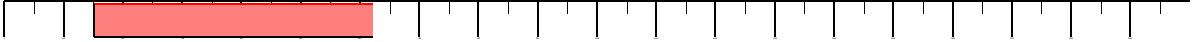
\includegraphics[scale=0.1]{chronogrames/4.jpeg}};
  \node (1) at (1,3){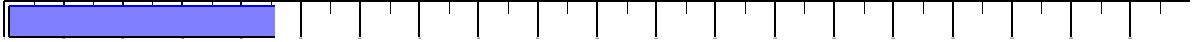
\includegraphics[scale=0.1]{chronogrames/1.jpeg}};
  \node (2) at (1,7){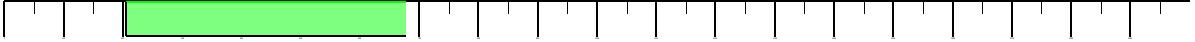
\includegraphics[scale=0.1]{chronogrames/5.jpeg}};
  \node (2) at (4,5){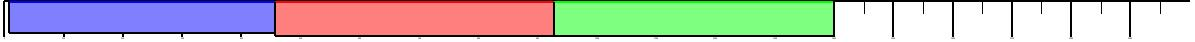
\includegraphics[scale=0.15]{chronogrames/6.jpeg}};
\end{tikzpicture}
}

Deterministic sending
\end{frame}


\begin{frame}{Tools}
  \centering
  
\scalebox{0.5}{
\begin{tikzpicture}
    \SetGraphUnit{5}
  \tikzstyle{VertexStyle}=[shape = circle, draw, minimum size = 50pt]
  \Vertex[x=0,y=0]{l3}
  \Vertex[x=0,y=4]{l2}
  \Vertex[x=0,y=8]{l1}
  
  \Vertex[x=16,y=0]{s3}
  \Vertex[x=16,y=4]{s2}
  \Vertex[x=16,y=8]{s1}
  
  \Vertex[x=4,y=4]{SL}
  \Vertex[x=12,y=4]{SS}  
  \tikzset{
  EdgeStyle/.append style = {<-,green} }
  \Edge[label = $a_1$](s1)(SS)
  \Edge[label = $b_1$](SL)(l1)
  
  \tikzset{
  EdgeStyle/.append style = {blue} }
  \Edge[label = $a_2$](s2)(SS)
  \Edge[label = $b_2$](SL)(l2)
  
  \tikzset{
  EdgeStyle/.append style = {red} }
  \Edge[label = $a_3$](s3)(SS)
  \Edge[label = $b_3$](SL)(l3)
  
  \tikzset{
  EdgeStyle/.append style = {black} }
  \Edge(SS)(SL)

  \node (0) at (1,-1){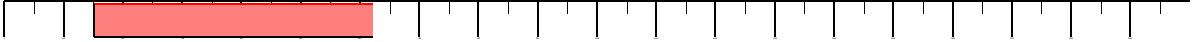
\includegraphics[scale=0.1]{chronogrames/4.jpeg}};
  \node (1) at (1,3){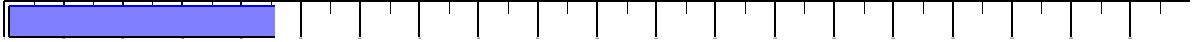
\includegraphics[scale=0.1]{chronogrames/1.jpeg}};
  \node (2) at (1,7){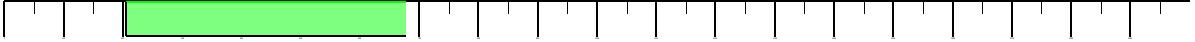
\includegraphics[scale=0.1]{chronogrames/5.jpeg}};
  \node (2) at (4,5){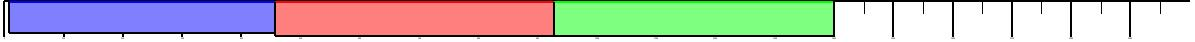
\includegraphics[scale=0.15]{chronogrames/6.jpeg}};
  \node (2) at (15,-1){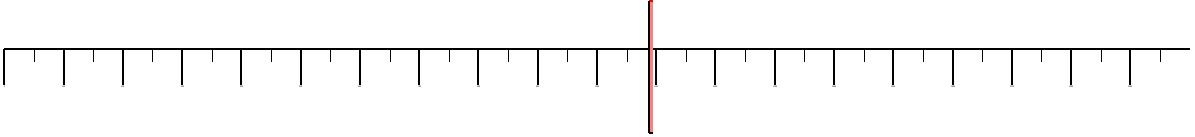
\includegraphics[scale=0.1]{chronogrames/7.jpeg}};
  \node (2) at (15,3){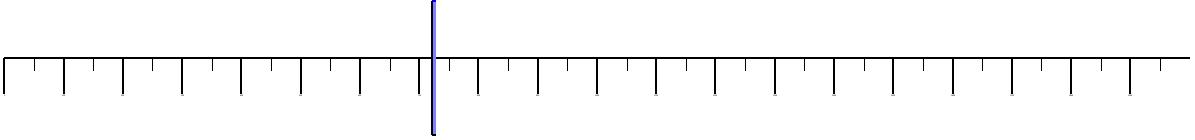
\includegraphics[scale=0.1]{chronogrames/8.jpeg}};
  \node (2) at (15,7){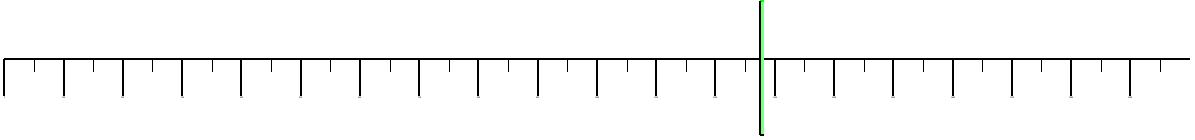
\includegraphics[scale=0.1]{chronogrames/9.jpeg}};
\end{tikzpicture}
}

Deterministic sending
\end{frame}




\begin{frame}{Tools}
  \centering
  
\scalebox{0.5}{
\begin{tikzpicture}
    \SetGraphUnit{5}
  \tikzstyle{VertexStyle}=[shape = circle, draw, minimum size = 50pt]
  \Vertex[x=0,y=0]{l3}
  \Vertex[x=0,y=4]{l2}
  \Vertex[x=0,y=8]{l1}
  
  \Vertex[x=16,y=0]{s3}
  \Vertex[x=16,y=4]{s2}
  \Vertex[x=16,y=8]{s1}
  
  \Vertex[x=4,y=4]{SL}
  \Vertex[x=12,y=4]{SS}  
  \tikzset{
  EdgeStyle/.append style = {->,green} }
  \Edge[label = $a_1$](s1)(SS)
  \Edge[label = $b_1$](SL)(l1)
  
  \tikzset{
  EdgeStyle/.append style = {blue} }
  \Edge[label = $a_2$](s2)(SS)
  \Edge[label = $b_2$](SL)(l2)
  
  \tikzset{
  EdgeStyle/.append style = {red} }
  \Edge[label = $a_3$](s3)(SS)
  \Edge[label = $b_3$](SL)(l3)
  
  \tikzset{
  EdgeStyle/.append style = {black} }
  \Edge(SS)(SL)

 
  \node (2) at (15,-1){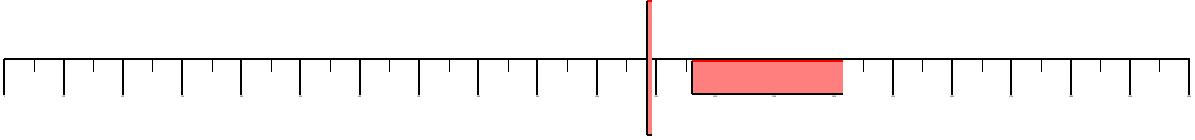
\includegraphics[scale=0.15]{chronogrames/19.jpeg}};
  \node (2) at (15,3){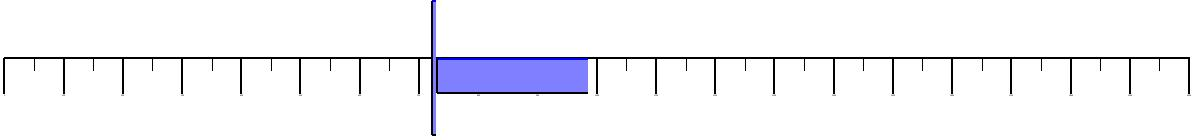
\includegraphics[scale=0.15]{chronogrames/17.jpeg}};
  \node (2) at (15,7){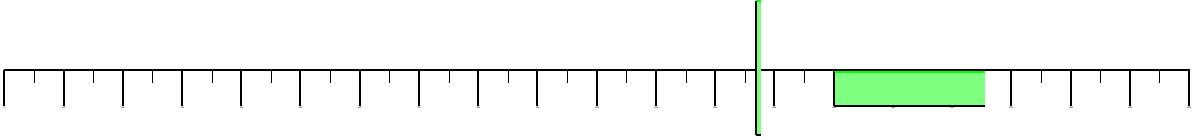
\includegraphics[scale=0.15]{chronogrames/18.jpeg}};
  \node (2) at (11,5){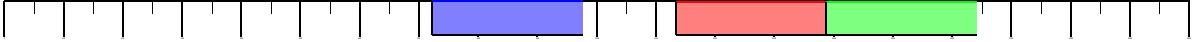
\includegraphics[scale=0.1]{chronogrames/20.jpeg}};
\end{tikzpicture}
}

Deterministic sending, waiting times.

$T_i = 2(RRH \rightarrow BBU) +$ waiting time.
\end{frame}
\end{subsection}
\end{section}

\begin{section}{Proposed heuristics}

\begin{frame}{Trivial case}
\centering
\scalebox{0.5}{
  \begin{tikzpicture}
    \SetGraphUnit{5}
  \tikzstyle{VertexStyle}=[shape = circle, draw, minimum size = 50pt]
  \Vertex[x=0,y=0]{l3}
  \Vertex[x=0,y=4]{l2}
  \Vertex[x=0,y=8]{l1}
  
  \Vertex[x=16,y=0]{s3}
  \Vertex[x=16,y=4]{s2}
  \Vertex[x=16,y=8]{s1}
  
  \Vertex[x=4,y=4]{SL}
  \Vertex[x=12,y=4]{SS}  
  \tikzset{
  EdgeStyle/.append style = {<-,green} }
  \Edge[label = 0](s1)(SS)
  \Edge[label = $b_1$](SL)(l1)
  
  \tikzset{
  EdgeStyle/.append style = {blue} }
  \Edge[label = 0](s2)(SS)
  \Edge[label = $b_2$](SL)(l2)
  
  \tikzset{
  EdgeStyle/.append style = {red} }
  \Edge[label = 0](s3)(SS)
  \Edge[label = $b_3$](SL)(l3)
  
  \tikzset{
  EdgeStyle/.append style = {black} }
  \Edge(SS)(SL)
\end{tikzpicture}
}

  \begin{itemize}
  \item Scheduling all messages following each others
  \item No waiting times
  \end{itemize}
\end{frame}

\begin{frame}{Shortest Longest}
\centering
\scalebox{0.5}{
  \begin{tikzpicture}
    \SetGraphUnit{5}
  \tikzstyle{VertexStyle}=[shape = circle, draw, minimum size = 50pt]
  \Vertex[x=0,y=0]{l3}
  \Vertex[x=0,y=4]{l2}
  \Vertex[x=0,y=8]{l1}
  
  \Vertex[x=16,y=0]{s3}
  \Vertex[x=16,y=4]{s2}
  \Vertex[x=16,y=8]{s1}
  
  \Vertex[x=4,y=4]{SL}
  \Vertex[x=12,y=4]{SS}  
  \tikzset{
  EdgeStyle/.append style = {<-,green} }
 
 
   \Edge[label = $a_1$](s1)(SS)
  
  \tikzset{
  EdgeStyle/.append style = {blue} }
 
  
    \Edge[label = $a_2$](s2)(SS)
  
  \tikzset{
  EdgeStyle/.append style = {red} }

 
     \Edge[label = $a_3$](s3)(SS)
  
  \tikzset{
  EdgeStyle/.append style = {black} }
 
  \Edge(SS)(SL)
   \Edge[label = $b_1$](SL)(l1)
   \Edge[label = $b_3$](SL)(l3)
 \Edge[label = $b_2$](SL)(l2)
   
\end{tikzpicture}
}

 $a_1 < a_2 < a_3$\\
 Send the messages from shortest route to the longest
 \begin{itemize}
 \item No collisions.
  \item Given period.
  \end{itemize}
\end{frame}


\begin{frame}{Longest Shortest Greedy (LSG)}

   \centering
  \scalebox{0.5}{
  
\begin{tikzpicture}
  \SetGraphUnit{5}
  \tikzstyle{VertexStyle}=[shape = circle, draw, minimum size = 50pt]
  \Vertex[x=0,y=0]{l3}
  \Vertex[x=0,y=4]{l2}
  \Vertex[x=0,y=8]{l1}
  
  \Vertex[x=16,y=0]{s3}
  \Vertex[x=16,y=4]{s2}
  \Vertex[x=16,y=8]{s1}
  
  \Vertex[x=4,y=4]{SL}
  \Vertex[x=12,y=4]{SS}  
  \tikzset{
  EdgeStyle/.append style = {<-,green} }
  \Edge[label = $a_1$](s1)(SS)
  \Edge[label = $b_1$](SL)(l1)
  
  \tikzset{
  EdgeStyle/.append style = {blue} }
  \Edge[label = $a_2$](s2)(SS)
  \Edge[label = $b_2$](SL)(l2)
  
  \tikzset{
  EdgeStyle/.append style = {red} }
  \Edge[label = $a_3$](s3)(SS)
  \Edge[label = $b_3$](SL)(l3)
  
  \tikzset{
  EdgeStyle/.append style = {black} }
  \Edge(SS)(SL)
\end{tikzpicture}
  
  }
  
  \begin{itemize}
  \item SL: Scheduling all messages from the one using the longest route to the one using the shortest.
  \item SS: 
    \begin{enumerate}
    \item Send the first message able to be sent.
    \item After each sending, among the messages able to be sent, send the one using the longest route.
    \end{enumerate}

  \end{itemize}

\end{frame}

% 
% \begin{frame}{Limits}
%     
%   \centering
%   \scalebox{0.5}
%   {
% \begin{tikzpicture}
%   \SetGraphUnit{5}
%    \tikzstyle{VertexStyle}=[shape = circle, draw, minimum size = 50pt]
%   \Vertex[x=0,y=0]{l3}
%   \Vertex[x=0,y=4]{l2}
%   \Vertex[x=0,y=8]{l1}
%   
%   \Vertex[x=16,y=0]{s3}
%   \Vertex[x=16,y=4]{s2}
%   \Vertex[x=16,y=8]{s1}
%   
%   \Vertex[x=4,y=4]{SL}
%   \Vertex[x=12,y=4]{SS}
%     
%   \tikzset{
%   EdgeStyle/.append style = {<-,green} }
%   \Edge[label = 687](s1)(SS)
%   \Edge[label = 256](SL)(l1)
%   
%   \tikzset{
%   EdgeStyle/.append style = {blue} }
%   \Edge[label = 288](s2)(SS)
%   \Edge[label = 633](SL)(l2)
%   
%   \tikzset{
%   EdgeStyle/.append style = {red} }
%   \Edge[label = 329](s3)(SS)
%   \Edge[label = 193](SL)(l3)
%   
%   \tikzset{
%   EdgeStyle/.append style = {black} }
%   \Edge(SS)(SL)
% \end{tikzpicture}
% 
%   }
%   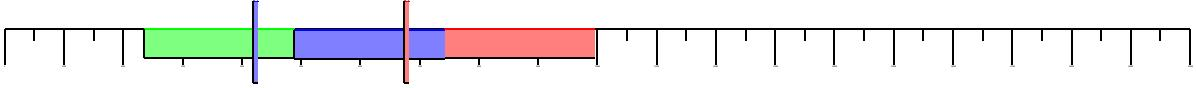
\includegraphics[scale = 0.2]{chronogrames/16.jpeg}
%   
%   $T_{max}$ = 4022 slots - Longest route delay *2 = 3268
%   
%   Optimal by splitting the emissions
% \end{frame}

\end{section}
\begin{section}{Performance Evaluations}
  
 \begin{frame}{Inputs}
 
 \centering
   \begin{tabular}{|c|c|c|}
   \hline
    Links capacity & 10Gbps & -\\
    \hline
    Flow/RRH & 1.228Gb/s & 2500 slots/ms\\
    \hline
    Flow max ($l_{max}$) & 7 & - \\
    \hline
    Considered Range & 0-5km & 2000 slots\\
    \hline
    Period & 1ms & 19500 slots\\
    \hline
    Deadline & 3ms (-2.6ms) & 7800 slots\\
    \hline
    \end{tabular}

 \end{frame}

\begin{frame}{Periods of algorithms without waiting times}
   \centering
  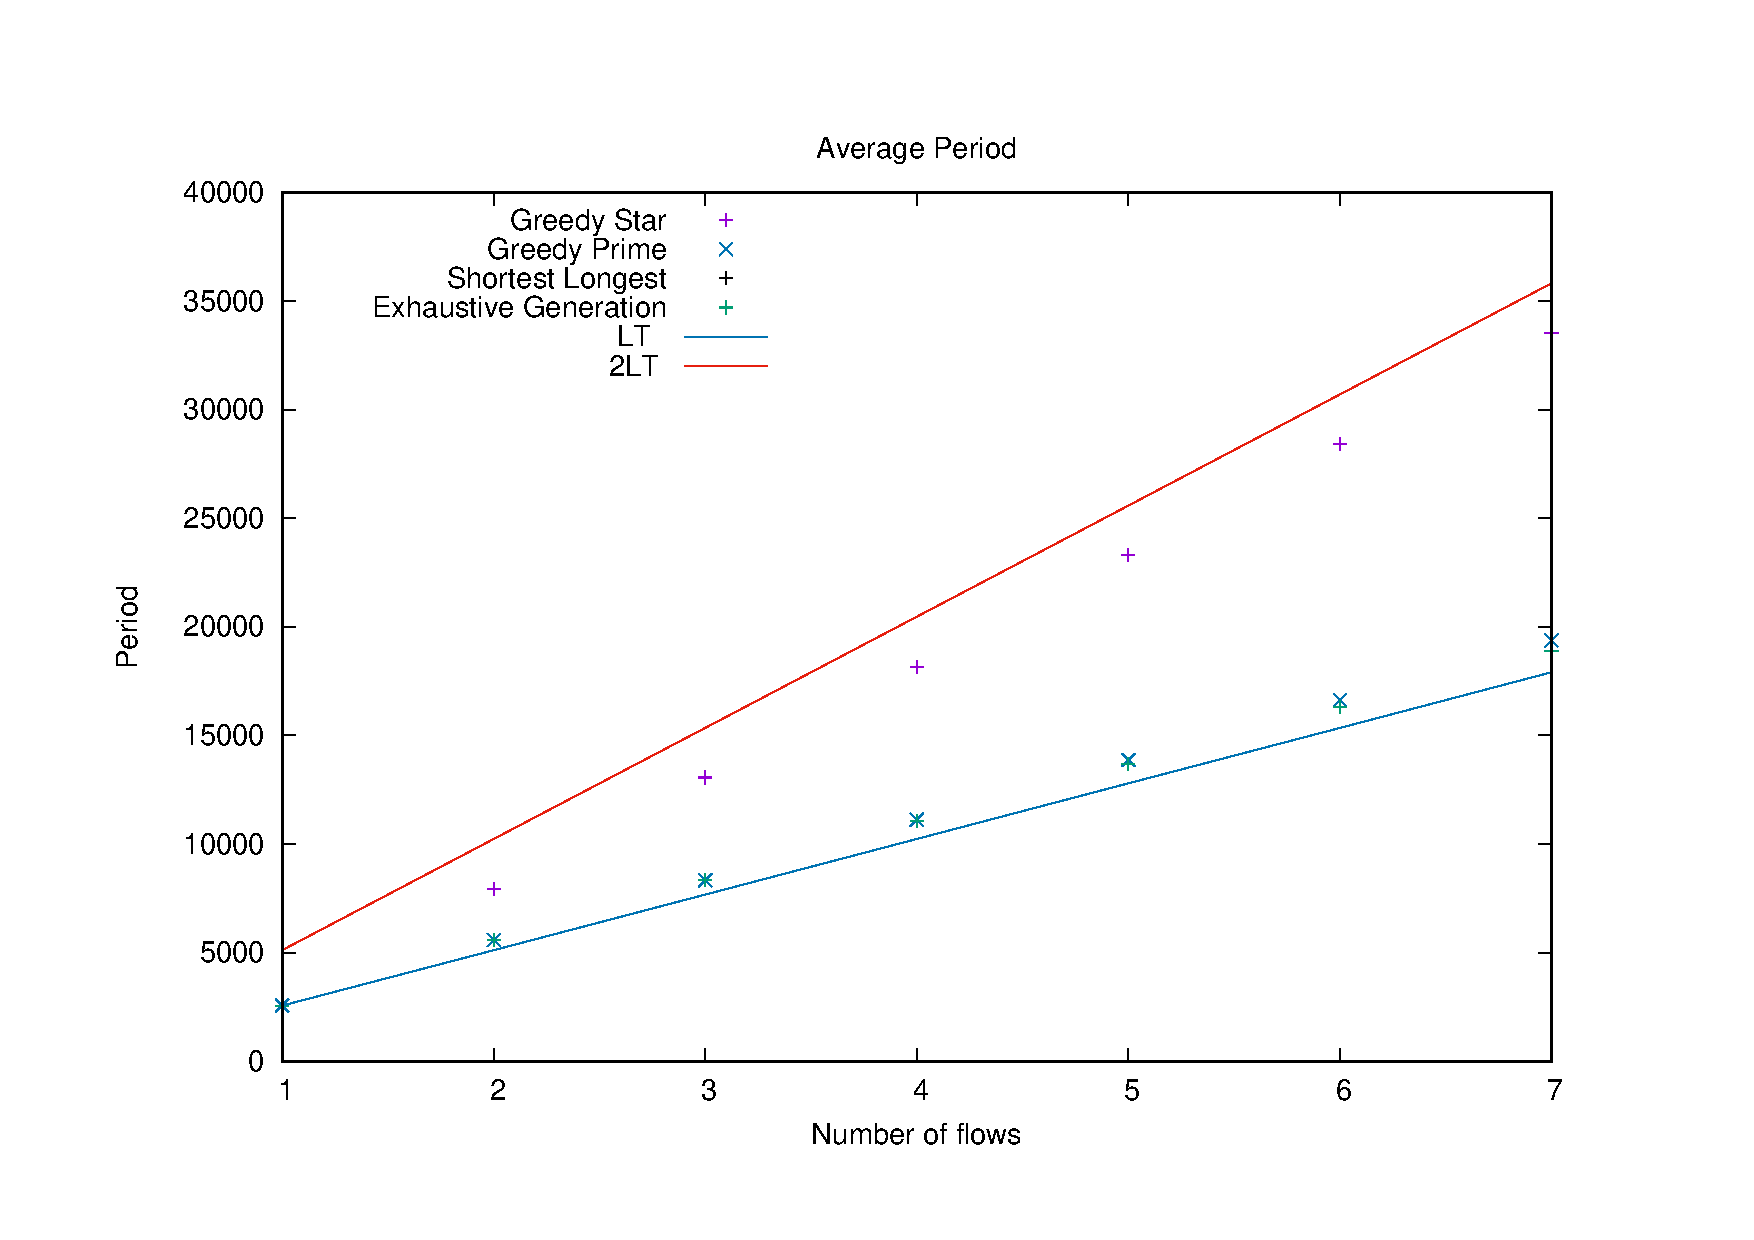
\includegraphics[scale=0.4]{window0.pdf}\\
\end{frame}

\begin{frame}{Longest Shortest Greedy versus Random}
   \centering
  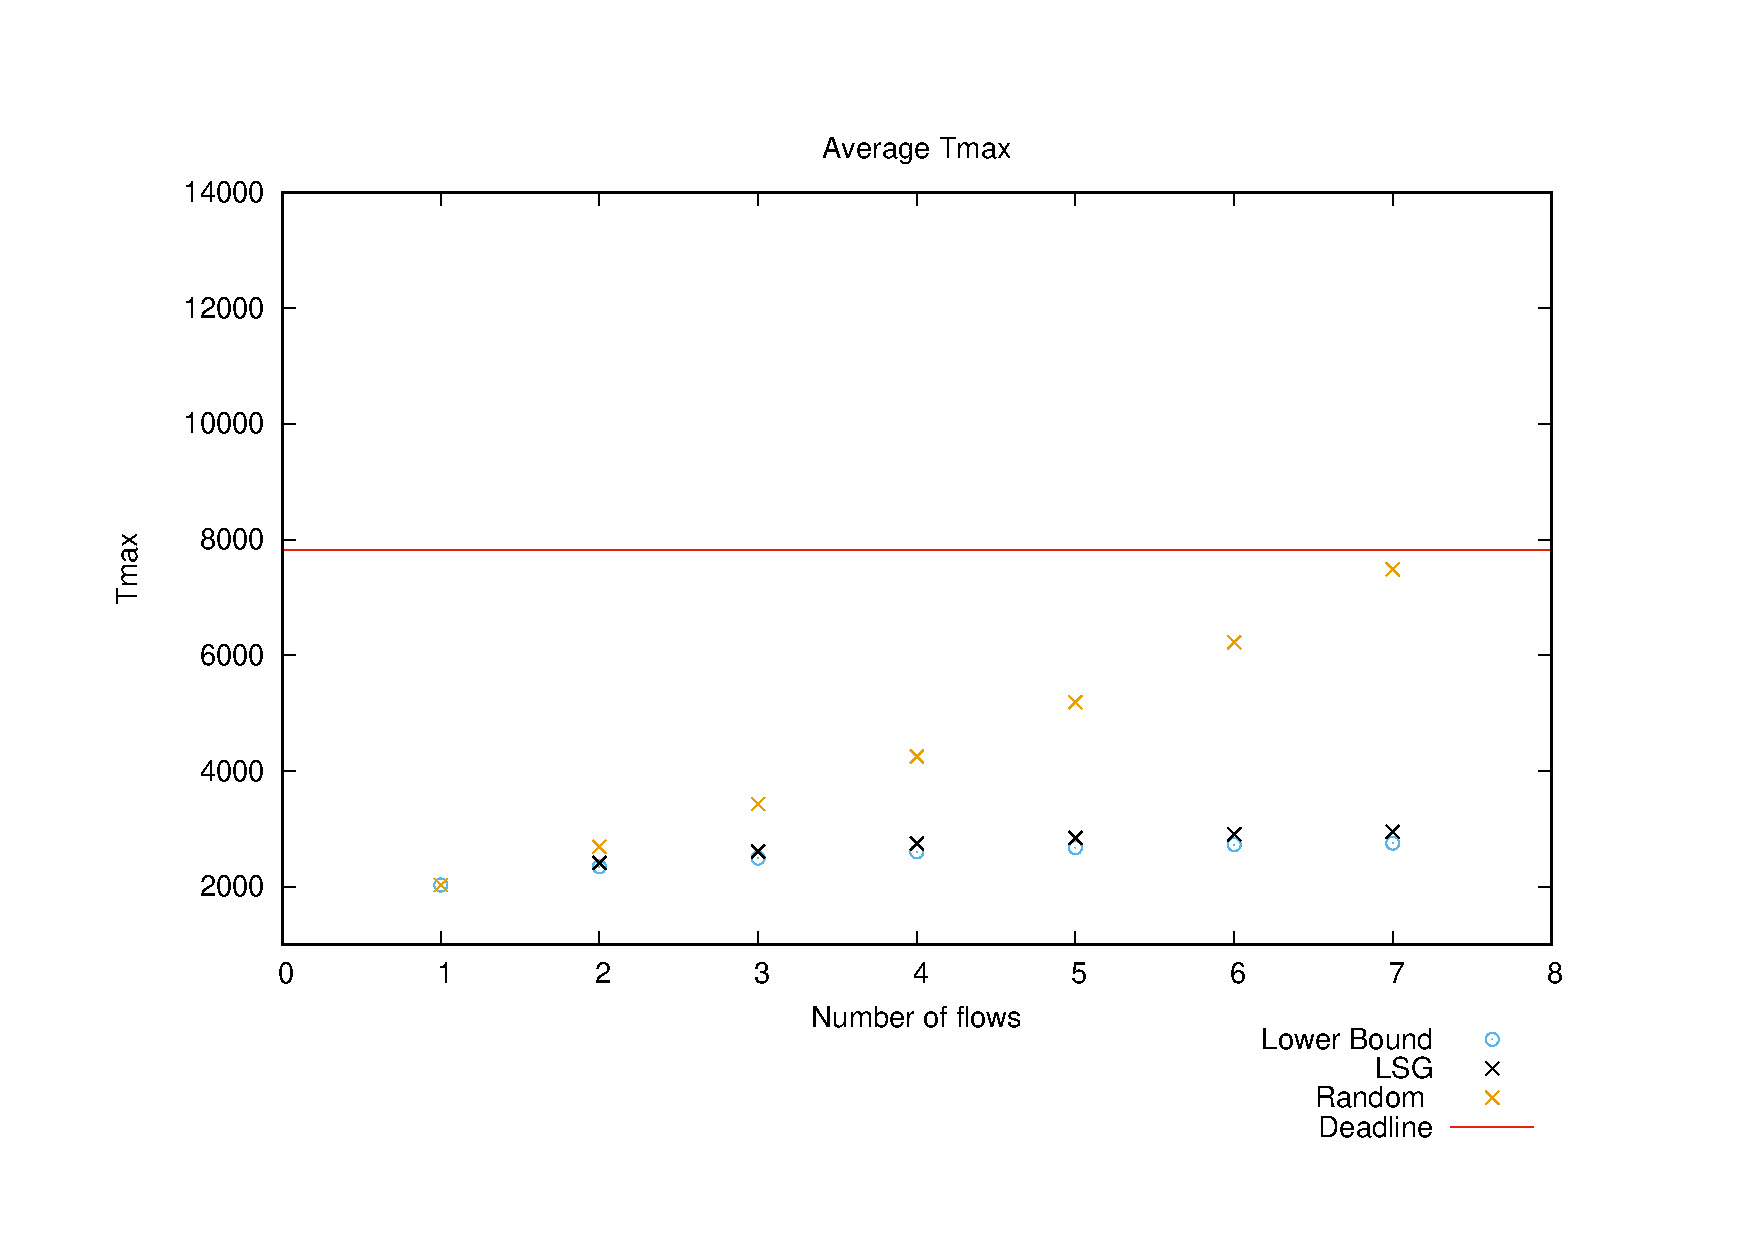
\includegraphics[scale=0.4]{tmax0.pdf}\\
\end{frame}

\begin{frame}{Longest Shortest Greedy versus Random}
   \centering
    \begin{tabular}{c c}
      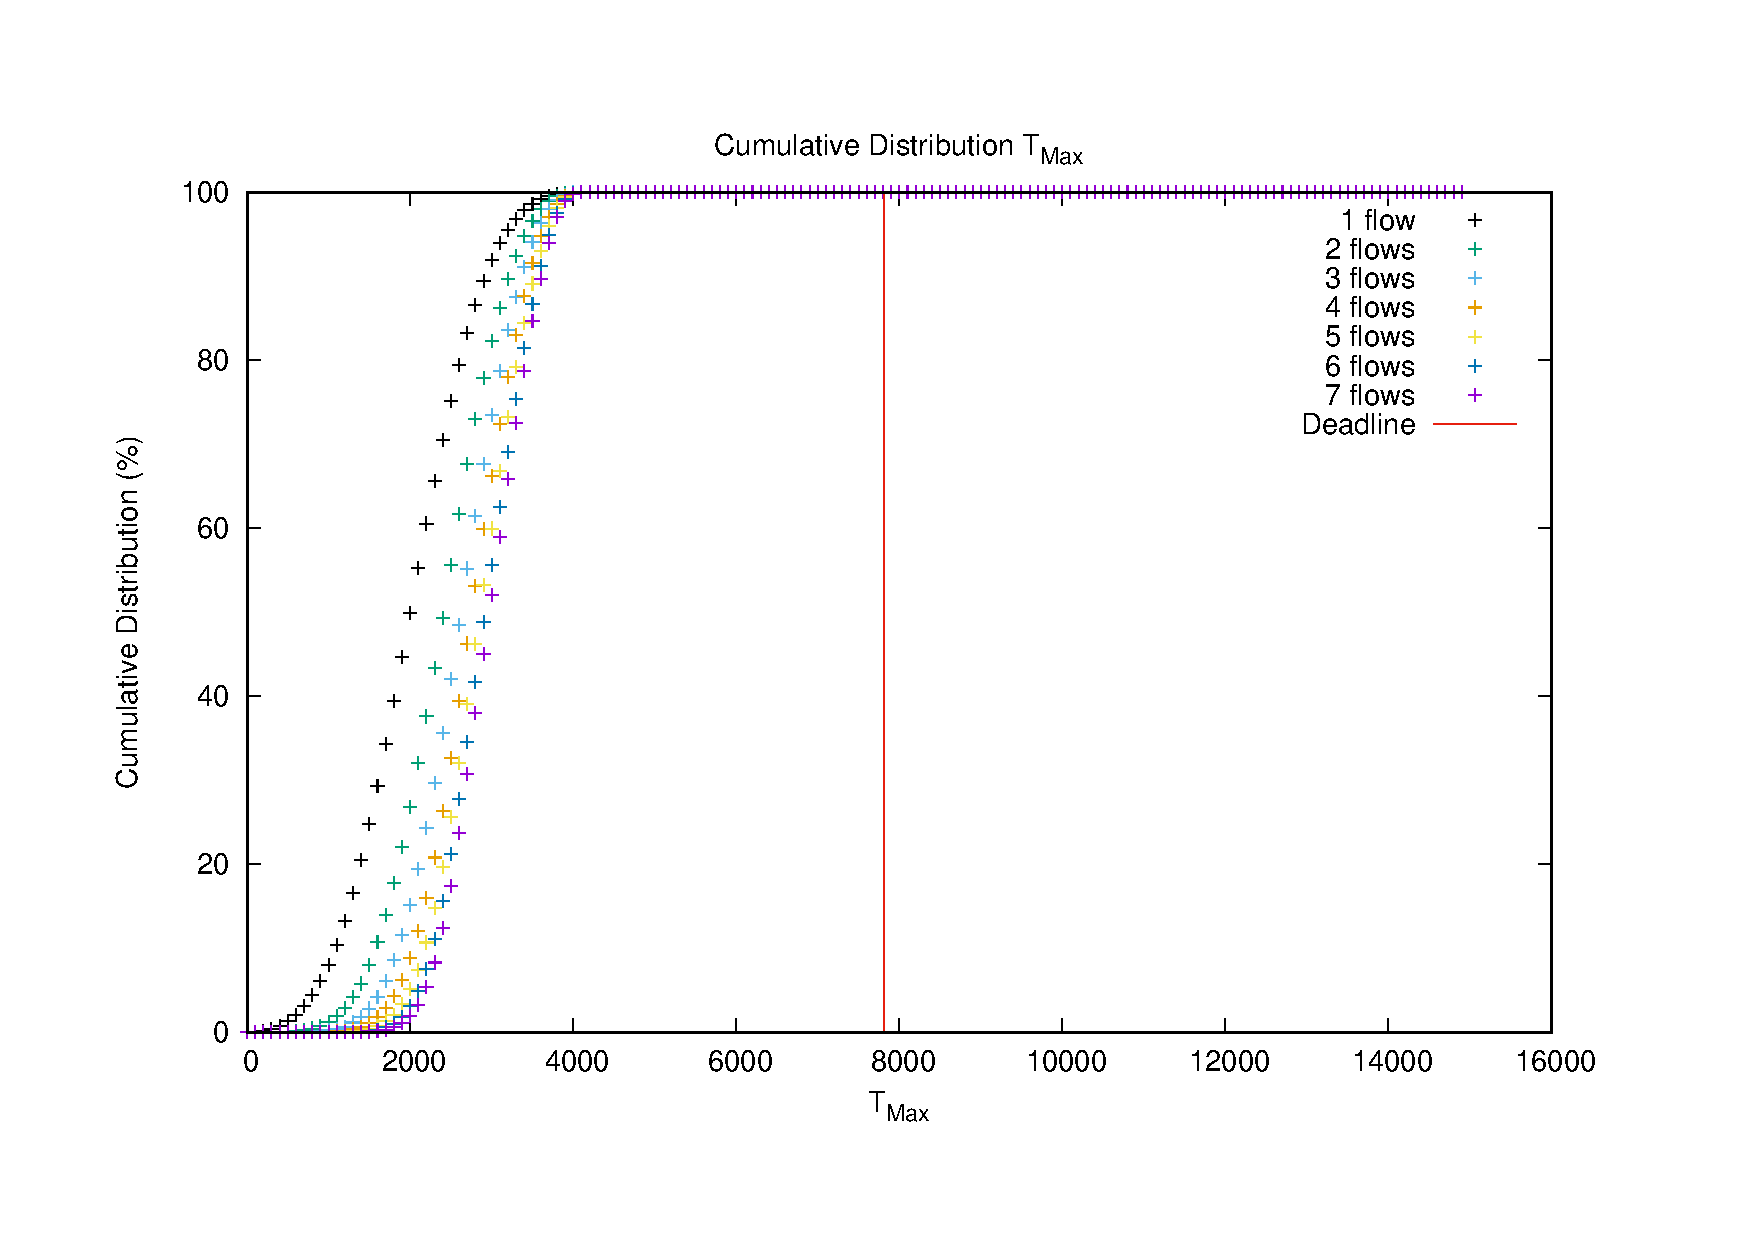
\includegraphics[scale=0.2]{distriscumul_longest.pdf} &  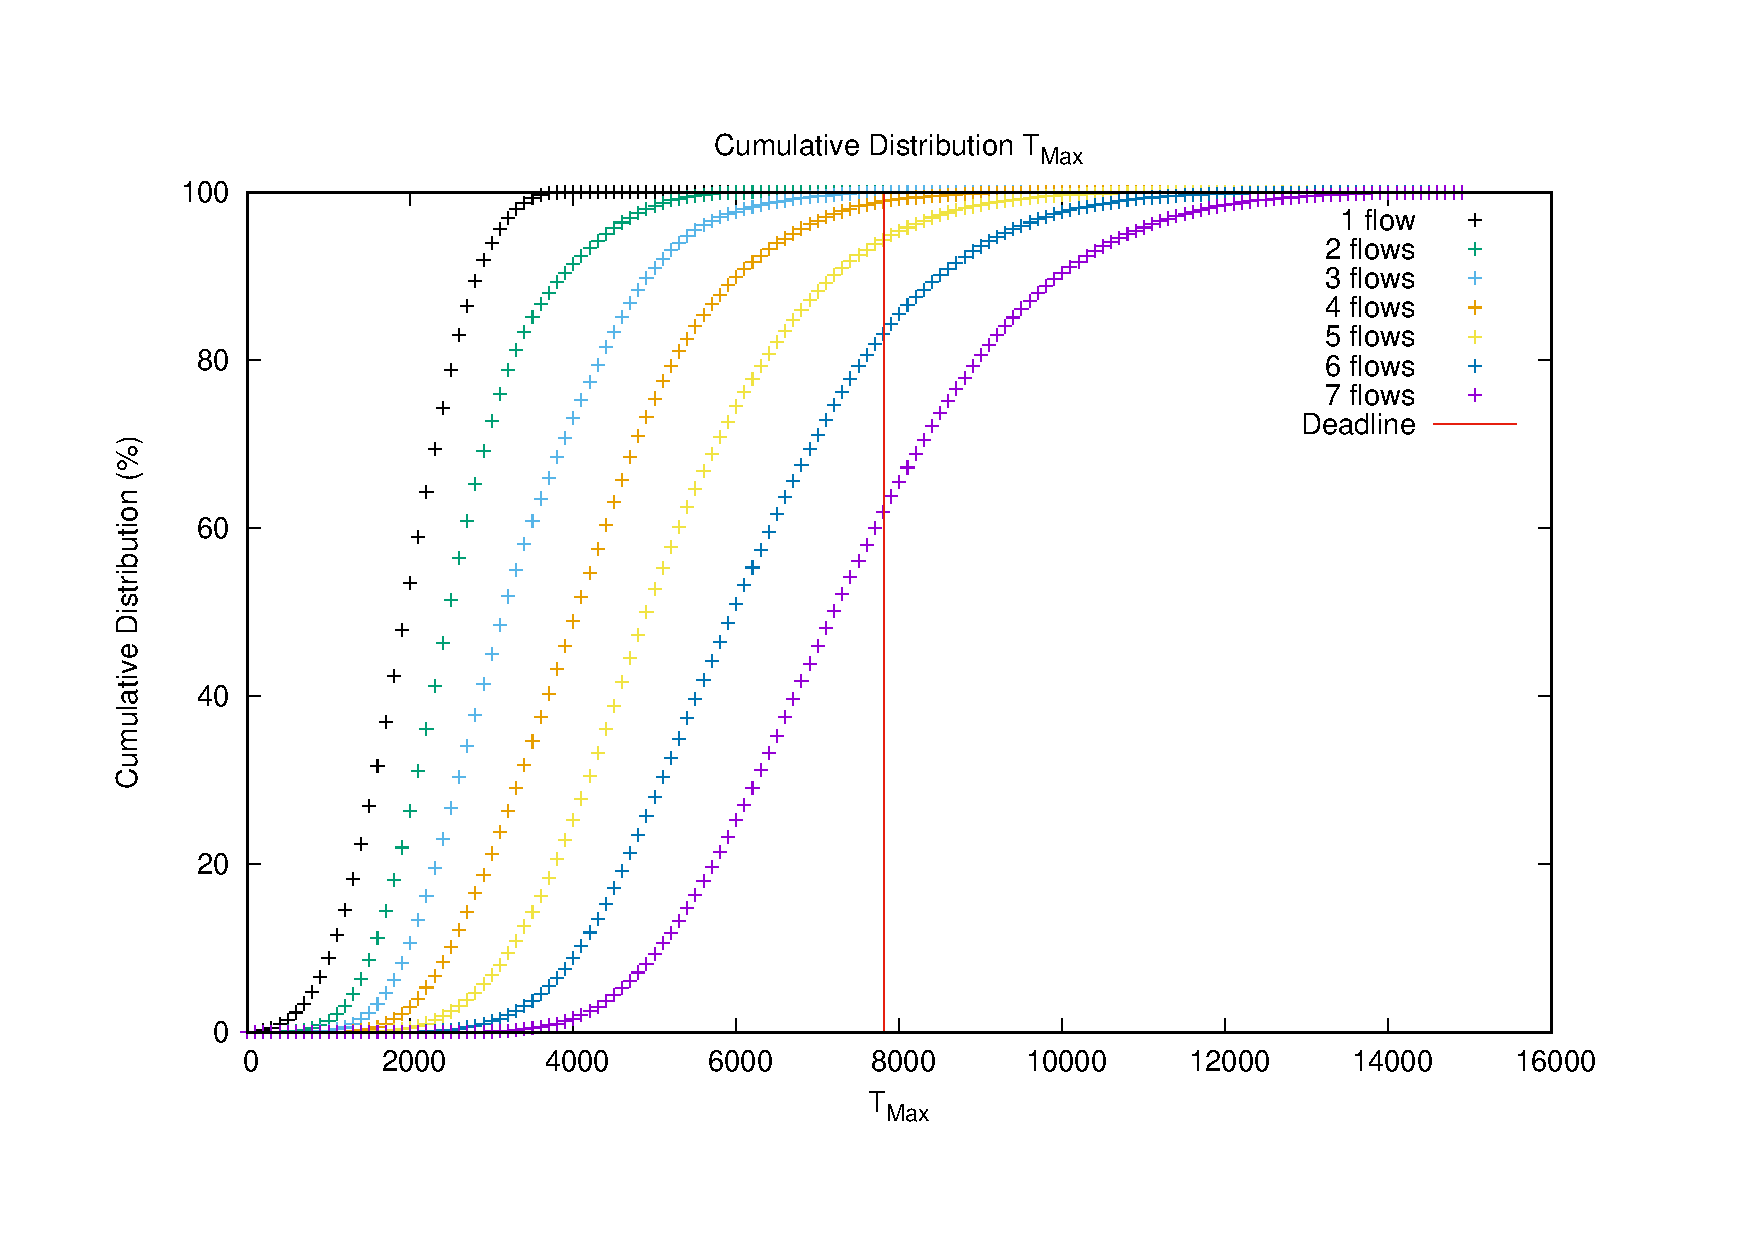
\includegraphics[scale=0.2]{distriscumul_random.pdf}\\
      LSG & Random \\
    \end{tabular}
     LSG $\rightarrow$ far from the deadline.
     
    Random $\rightarrow 10\%$ solutions with $T_{max} >$ deadline for 5 flows.

\end{frame}

\end{section}

\begin{section}{Conclusion}
 

\begin{frame}{Conclusion}

 \begin{block}{Some good results}
  Deterministic approach better than statistic.\\
    Optimal algorithm without waiting times for a reasonable load of the network (Shortest Longest). Good heuristic (LSG) when waiting times are allowed.
 \end{block}
 
  \begin{block}{but much improvements to do !}
    Better model, study of the others topologies, ...
 \end{block}

\end{frame}

\end{section}


\end{document}
